\documentclass[12pt,english]{article}
\usepackage[T1]{fontenc}
\usepackage[latin9]{inputenc}
\usepackage{amsmath}
\usepackage{graphicx}

\makeatletter
\usepackage[letterpaper,body={6.5in,9in}, head=34pt, foot=70pt]{geometry}
\usepackage{fancyhdr}

\pdfpagewidth 8.5in
\pdfpageheight 11in

\pagestyle{fancy}
\headheight 35pt

\rhead{Fall 2021}
\chead{}
\lhead{Sunny Lee \quad MATH 3700 Operations Research}
\renewcommand{\footrulewidth}{0.4pt}
\rfoot{\thepage}
\cfoot{}
\lfoot{Wentworth Institute of Technology}

\usepackage{multicol}

\makeatother

\usepackage{babel}
\begin{document}

\begin{enumerate}
    \item 
    \begin{gather*}
        \text{minimize } x_1^2 + x_2^2 \\
        \text{subject to } 2x_1x_2 = 3
    \end{gather*}
    The contour map of the objective function as well as the constraint: \\
    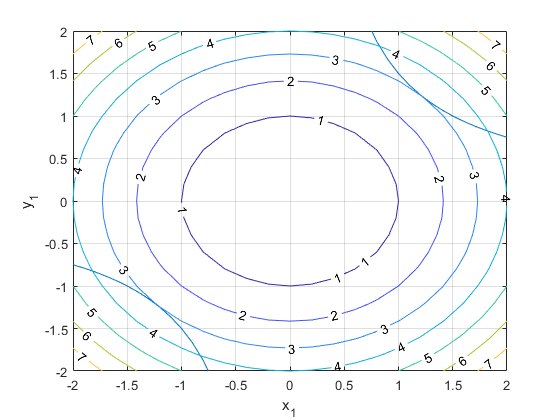
\includegraphics{a.png}
    \begin{enumerate}
        \item 
        The Lagrangian function in our case is: 
        \begin{gather*}
            \mathcal{L}(x_1, x_2, \lambda) = f(x_1, x_2) + \lambda h(x_1, x_2) = 
            x_1^2 + x_2^2 + 2\lambda x_1x_2 - 3\lambda
        \end{gather*}
        \item
        \begin{gather*}
            \nabla \mathcal{L} = 
            \begin{bmatrix}
                2x_1 + 2\lambda x_2\\
                2x_2+2\lambda x_1 \\
                2x_1x_2 - 3
            \end{bmatrix}
        \end{gather*}
        \item 
        Setting the gradient equal to zero, we are left with the system of equations: 
        \[
        \begin{cases}
            2x_1 + 2\lambda x_2 = 0 \\
            2x_2 + 2\lambda x_1 = 0 \\
            2x_1x_2-3 = 0
        \end{cases}
        \]
        Using the third equation, we obtain $x_1 = \frac{3}{2x_2}$. Then, 
        \begin{gather*}
            2(\frac{3}{2x_2}) + 2\lambda x_2 = 0\\
            \frac{3}{x_2} = -2\lambda x_2\\
            \lambda = \frac{-3}{2x_2^2}
        \end{gather*}
        then,
        \begin{gather*}
            2x_2 + 2(\frac{-3}{2x_2^2})(\frac{3}{2x_2}) = 0\\
            2x_2 = \frac{9}{2x_2^3}\\
            x_2^4 = \frac{9}{4}\\
            x_2 = \sqrt{\frac{3}{2}}
        \end{gather*}
        Thus, $\lambda = \frac{-3}{2\frac{3}{2}} = -1$ and 
        $x_1 = \frac{3}{2\sqrt{\frac{3}{2}}}$ and we have a solution at the point
        $(\frac{3}{2\sqrt{\frac{3}{2}}}, \sqrt{\frac{3}{2}})$ which gives us a value
        of $3$. 
        \item 
        We can check our answer by taking the gradient of the objective function 
        and comparing it to the gradient of our restriction at the point: 
        \begin{gather*}
            \nabla (x_1^2 + x_2^2) = 
            \begin{bmatrix}
                2x_1\\
                2x_2
            \end{bmatrix}, 
            \nabla (2x_1x_2 - 3) = 
            \begin{bmatrix}
                2x_2 \\
                2x_1
            \end{bmatrix}
        \end{gather*}
        Since
        \begin{gather*}
            2x_1 = 2\left(\frac{3}{2\sqrt(\frac{3}{2})}\right) = \frac{3}{\sqrt{\frac{3}{2}}} = 
            3\frac{\sqrt{2}}{\sqrt{3}}\cdot \frac{\sqrt{2}\sqrt{3}}{\sqrt{2}\sqrt{3}} = 
            3\frac{2\sqrt{3}}{3\sqrt{2}} = 2\frac{\sqrt{3}}{\sqrt{2}} = 2\sqrt{\frac{3}{2}} = 2x_2
        \end{gather*}
        we obtain $2x_1 = 2x_2$ and thus the gradients of the two functions are parallel. 
        Thus, this is an optimal solution to our problem.  
    \end{enumerate}
    \pagebreak
    \item 
    \begin{enumerate}
        \item 
        $$f(x_1, x_2)  = 8x_1+12x_2+x_1^2-2x_2^2$$
        \[
        \nabla f(\mathbf{x}^*) = 
        \begin{bmatrix}
            \frac{\partial f}{\partial x_1} \\
            \frac{\partial f}{\partial x_2}
        \end{bmatrix}
        =
        \begin{bmatrix}
            8 + 2x_1\\
            12 - 4x_2
        \end{bmatrix}
        \]
        Since both partial derivatives are linear, we will only have one stationary point 
        at $x_1 = -4$ and $x_2 = -6$
        \item 
        Calculating the Hessian: 
        \[
            H = \nabla^2 f(\mathbf{x}) = 
            \begin{bmatrix}
                \frac{\partial^2 f}{\partial x_1^2} & \frac{\partial^2 f}{\partial x_1 x_2}\\
                \frac{\partial^2 f}{\partial x_2 x_1} & \frac{\partial^2 f}{\partial x_2^2}
            \end{bmatrix}
            =
            \begin{bmatrix}
                2 & 0 \\
                0 & -4
            \end{bmatrix}
        \]
        Taking the determinant of the Hessian: $det(H) = 2(-4) + 0\cdot 0 = -8$. Since 
        the determinant is negative, we have that our stationary point is a sadddle point. 
        \item 
        Since in the objective function we have the two terms $x_1^2 - 2x_2^2$, 
        we would expect our contour lines to be hyperbolas. 
    \end{enumerate}
\end{enumerate}

\end{document}